\documentclass[journal]{IEEEtran}
\usepackage[utf8]{inputenc}
\usepackage{cite}
\usepackage{amsmath,amssymb,amsfonts}
\usepackage{algorithmic}
\usepackage{graphicx}
\usepackage{textcomp}
\usepackage{xcolor}
\usepackage{tabularx}
\usepackage{stfloats}
\usepackage{booktabs}
\usepackage[hidelinks]{hyperref}

\def\BibTeX{{\rm B\kern-.05em{\sc i\kern-.025em b}\kern-.08em
    T\kern-.1667em\lower.7ex\hbox{E}\kern-.125emX}}
\begin{document}
\title{Anomaly-Aware Battery Dispatch: A VAE-Based Detection Pipeline for Robust Energy Market Optimization}

\author{\IEEEauthorblockN{Keshav Aggarwal}
\IEEEauthorblockA{\textit{Student, Department of Computer Science and Engineering} \\
\textit{Thapar Institute of Engineering and Technology}\\
Patiala, India \\
ka9812204392@gmail.com}
}
\maketitle

\begin{abstract}
Battery energy storage systems (BESS) participating in energy markets are increasingly exposed to adversarial price manipulation, where artificial price spikes are injected into market signals to induce suboptimal charging and discharging decisions. Existing state-of-the-art strategies either ignore such price events entirely, leaving the system fully exposed to manipulation, or apply blanket penalties that forfeit legitimate trading opportunities during genuine market stress. This paper proposes a two-stage framework that combines a Variational Autoencoder (VAE) with an ensemble of Isolation Forest  (iForest) and Local Outlier Factor (LOF) detectors to classify hourly price deviations as either genuine market events or synthetic injections. The resulting anomaly signal is integrated under three operating regimes: baseline (anomaly-agnostic), penalized (anomaly-averse), and opportunistic (anomaly-adaptive). The genuine-versus-synthetic classifier achieves an $F_1$ score of $0.5859$ and a precision of $0.9615$ on 727 anomalous hours evaluated against honest ground truth derived from injected spike positions. Experiments on three years of California electricity price data demonstrate that the opportunistic regime achieves a $0.53\%$ profit improvement over the anomaly-agnostic baseline under adversarial conditions while maintaining comparable clean-market performance. A robustness sweep across 15 spike magnitude and duration configurations confirms consistent detection rates scaling from $10.7\%$ at $1.5\times$ magnitude to $71.0\%$ at $8\times$ magnitude. Explainability of dispatch decisions is further supported by adapting Gradient-weighted Class Activation Mapping (Grad-CAM) to the temporal VAE setting, providing market operators with a human-readable audit trail for every charge and discharge decision.
\end{abstract}

\begin{IEEEkeywords}
battery energy storage, variational autoencoder, anomaly detection, energy market optimization, adversarial price injection, State of Charge (SoC), Grad-CAM, arbitrage, sensitivity analysis
\end{IEEEkeywords}
   
\section{Introduction}

Battery energy storage systems are emerging as critical assets in modern peer-to-peer (P2P) energy markets, providing services such as price trading, frequency regulation, and spinning reserve. As market participants increasingly rely on automated algorithms that respond to real-time price signals, these systems become attractive targets for adversarial manipulation: artificial price spikes are injected into market signals, inducing suboptimal charging and discharging decisions that reduce prosumer revenue and destabilize grid operations.

The pricing nodes in Southern California, one of the most actively traded hubs in the energy market, serve as a representative dataset for this problem, given its high price volatility and exposure to both renewable unpredictability and strategic bidding behavior. Existing dispatch strategies address this vulnerability poorly. Anomaly-agnostic approaches treat all price signals as legitimate. They are fully exposed to manipulation, while blanket anomaly-penalized strategies avoid trading during all unusual price events, forfeiting legitimate revenue during genuine market stress events such as heatwaves or supply shortfalls.

Recent advances in deep generative models and unsupervised anomaly detection offer a promising path forward. VAEs have demonstrated strong capability in learning compact latent representations of normal temporal patterns, making reconstruction error a natural signal for detecting anomalies in time-series data. Methods such as iForest and LOF complement this by capturing anomalies from a statistical density perspective, with each detector sensitive to different aspects of price irregularity. However, anomaly detection alone is insufficient for dispatch decisions: a spike flagged as anomalous may be either a genuine market event worth exploiting or a synthetic injection that must be avoided. A classification layer that distinguishes genuine from adversarial anomalies based on persistence, mean reversion, and rate of change is, therefore, a necessary addition to any detection pipeline deployed in a live market setting.

\section{Related Work}

The problem addressed in this paper sits at the intersection of electricity price forecasting~\cite{Price_Forecasting}, anomaly detection in energy systems~\cite{AE_Anomaly}, and adversarial robustness in BESS dispatch~\cite{BESS}. While each area has developed substantial independent literature, the specific question of how anomaly classification translates into measurable dispatch profit under adversarial conditions remains largely unaddressed.

Early work on electricity price anomaly detection relied on statistical process control and threshold-based methods, flagging prices that exceeded a fixed multiple of a rolling mean or standard deviation. While computationally lightweight, these approaches lack the temporal context needed to distinguish a genuine demand spike from a brief manipulated injection, as both can produce similar single-hour deviations. Autoregressive models such as ARIMA and its variants improved on this by modeling expected prices as a function of history, with residuals serving as anomaly scores.

The introduction of deep learning models has substantially expanded detection capability. Long Short-Term Memory (LSTM) networks were applied to price forecasting, with reconstruction error used as an anomaly indicator, demonstrating sensitivity to multi-hour deviations that most statistical methods missed. More recently, VAE-based approaches have gained attention because the probabilistic latent space provides a principled measure of how far an observation lies from the learned normal distribution, rather than a purely deterministic reconstruction distance. Critically, however, the existing VAE literature on electricity prices treats detection as the terminal objective; cited works do not close the loop back to dispatch decisions, which this paper directly addresses.

Optimal dispatch has been extensively studied as both a stochastic and a deterministic optimization problem. Model predictive control frameworks formulate dispatch as a rolling program updated as new price forecasts arrive. Stochastic programming extensions account for forecast uncertainty by optimizing over scenario trees at the cost of significantly increased computational complexity. Reinforcement learning approaches have been proposed to learn dispatch policies directly from market interactions, with several studies reporting that Model Predictive Control baselines outperform them in volatile price environments.

What unites all of these formulations, however, is an assumption that the price signal is trustworthy. Adversarial injection is not modeled, and no mechanism exists to exploit or penalize anomalous prices based on their origin differentially. The framework proposed here extends the linear programming formulation with an anomaly-conditioned objective and constraint set, filling this gap without sacrificing the tractability and auditability that make linear programming-based dispatch preferable in regulated market contexts.

\section{System Architecture and Pipeline}
\label{sec:pipeline}

\subsection{Overview}
The proposed framework processes raw electricity price data through four stages: data ingestion, anomaly detection, spike classification, and adaptive dispatch, before producing a profit-maximizing charge/discharge schedule. Each stage is designed to be independent of the others: the anomaly detector can be swapped without modifying the optimizer, and the classification thresholds can be recalibrated for different market nodes without retraining the VAE. This modularity is deliberate, as operational energy systems require components that can be audited, updated, and replaced independently in response to changing market conditions or regulatory requirements.

\subsection{Stage 1 - Data Ingestion and Preprocessing}
The pipeline ingests hourly locational marginal prices from the SP15, NP15, and ZP26 nodes, along with four ancillary service markets: regulation up (RegUp), regulation down (RegDown), spinning reserve (Spin), and non-spinning reserve (NonSpin). To avoid repeated API calls across runs, all fetched data is stored immediately in a compressed CSV cache on first retrieval. Every subsequent run loads from this cache, which automatically restores datetime types and reduces execution time. A single aggregation step collapses the multi-node structure into a single hourly time series before passing the data downstream.

\noindent\textbf{Sample Data}

\begin{table*}[!h]
\centering
\caption{Sample market data by node and timestamp}
\label{tab:market_data}
\begin{tabular}{llrrr}
\hline
\textbf{datetime} & \textbf{node} & \textbf{SP15} & \textbf{NonSpin} & \textbf{RegDown} \\
\hline
2023-01-12 08:00:00 & TH\_NP15\_GEN-APND & 137.79688 & 0.27 & 7.99 \\
2023-01-12 08:00:00 & TH\_SP15\_GEN-APND & 138.44933 & 0.27 & 7.99 \\
2023-01-12 08:00:00 & TH\_ZP26\_GEN-APND & 135.07355 & 0.27 & 7.99 \\
2023-01-12 09:00:00 & TH\_NP15\_GEN-APND & 132.21107 & 0.27 & 7.99 \\
2023-01-12 09:00:00 & TH\_SP15\_GEN-APND & 132.93228 & 0.27 & 7.99 \\\hline
\end{tabular}
\end{table*}

\subsection{Stage 2 - Ensemble Anomaly Detection}
The anomaly detector is a three-member ensemble, each member contributing a distinct perspective on whether a given hourly price observation is normal or anomalous. The VAE, the primary member, is trained on the first 80\% of the time series using 24-hour input sequences. At inference time, hours the VAE struggles to reconstruct incur a high per-timestep reconstruction error, which forms the VAE's continuous anomaly score. The secondary members, iForest and LOF, are classical unsupervised outlier detectors that approach the problem from a density perspective using continuous \texttt{score\_samples()} rather than binary classification: prices in sparsely populated regions of the distribution receive higher anomaly scores regardless of temporal context. Importantly, all three detectors are fitted exclusively on the training split; the held-out test period is never used during fitting, ensuring no information leakage. The three continuous scores are combined into a single ensemble score in $[0, 1]$ via weighted summation with weights $0.5$, $0.3$, and $0.2$, respectively.

\subsection{Stage 3 - Genuine vs.\ Synthetic Spike Classification}
A high anomaly score alone is insufficient to determine how the dispatch optimizer should respond: a genuine demand surge caused by a heatwave and a synthetic price injection both produce high scores, but the correct dispatch response to each is opposite. The classification stage resolves this ambiguity by combining three behavioral signals into a continuous $is\_genuine$ score in $[0, 1]$. First, a persistence signal checks whether the elevated price persists across a rolling window; genuine market stress events typically sustain elevated prices for several consecutive hours. Second, a non-reversion signal measures how much the current price exceeds the forward rolling mean: genuine shocks remain elevated relative to their near-future mean, whereas synthetic injections revert sharply and fall below that mean quickly. Third, a rate-of-change signal captures near-instantaneous step jumps, which are a common signature of synthetic data injection but rare in real markets where price formation involves continuous participant bidding. Rather than a hard binary label, these three signals are combined with weights $0.4$, $0.3$, and $0.3$ respectively into the continuous $is\_genuine$ score, which the optimizer treats as a soft weight rather than an on/off switch. This probabilistic design allows the optimizer to hedge when classification confidence is low partially.

\subsection{Stage 4 - Anomaly-Adaptive Dispatch Optimization}
The dispatch optimizer is a linear program solved using the HiGHS solver via Pyomo. It selects an hourly charge and discharge schedule to maximize total operating profit subject to the battery's physical constraints: SoC evolves according to round-trip efficiency, discharge is bounded by available stored energy, and charge is bounded by remaining capacity. Transaction fees and per-cycle degradation costs are included in the objective to reflect real operational economics.

The three operating regimes differ only in how the anomaly signal modulates the sell constraint and objective coefficients. In the baseline regime, anomaly scores are ignored entirely. In the penalized regime, sell limits and effective price weights are reduced proportionally to the anomaly score, leading the battery to trade less aggressively whenever an anomaly is detected. In the opportunistic regime - the proposed method - the anomaly score is decomposed using the $is\_genuine$ weight: confirmed genuine spikes raise the sell limit and increase the effective sell price. In contrast, suspected synthetic spikes lower the sell limit. The degree of response in both directions is governed by the sensitivity parameter $\lambda \in [0, 1]$.

\subsection{Explainability via Temporal Grad-CAM}

To address the interpretability requirements that accompany any AI-assisted trading system operating in a regulated market, the framework adapts Gradient-weighted Class Activation Mapping (Grad-CAM) to the temporal VAE setting. In the original image classification context, Grad-CAM identifies which spatial regions of an input image most influenced the model's output by computing the gradient of the target class score with respect to the final feature map. Here, the same principle is applied across the temporal dimension: the gradient of the VAE's total reconstruction error with respect to each 24-hour input sequence identifies which hours the model found most anomalous and therefore most influential in shaping the dispatch signal. The resulting per-hour influence scores are aligned with the original hourly time axis and stored alongside the dispatch output, providing a market operator with a human-readable explanation of why the system chose to charge, discharge, or remain idle at any given hour.

\section{Model Equations and Parameters}

The battery SoC is updated according to

\begin{equation}
SOC_t = SOC_{t-1} + \left( buy_t \cdot e - \frac{sell_t}{e} \right) dt
\end{equation}

where charging and discharging are constrained by

\begin{equation}
sell_t \leq e \cdot SOC_{t-1}
\end{equation}

\begin{equation}
buy_t \cdot e \leq Capacity_{MWh} - SOC_{t-1}
\end{equation}

The maximum discharge power is limited by

\begin{equation}
sell_t \leq MaximumDispatchPower
\end{equation}

The objective is to maximize net revenue:

\begin{equation}
\max \sum_t \left(
sell_t \cdot price_t
-
buy_t \cdot price_t
-
cost \cdot (sell_t + buy_t)
\right)
\end{equation}

\begin{table}[!t]
\centering
\caption{Model Parameters and Variables}
\label{tab:model_params}
\begin{tabular}{ll}
\hline
Symbol & Description \\
\hline
$SOC_t$ & Battery SoC at time $t$ \\
$buy_t$ & Energy purchased at time $t$ \\
$sell_t$ & Energy sold at time $t$ \\
$e$ & Battery efficiency \\
$dt$ & Time interval duration \\
$Capacity_{MWh}$ & Maximum battery capacity \\
$price_t$ & Electricity market price at time $t$ \\
$cost$ & Transaction fee \\
\hline
\end{tabular}
\end{table}

\section{Dataset Description}

\subsection{Data Sources}
The dataset was obtained from the California Independent System Operator (CAISO) wholesale electricity market via the \texttt{gridstatus} API. Three major trading hubs were selected to represent geographically diverse regions of the California power system:

\begin{itemize}
    \item \textbf{SP15} (South Path 15 Trading Hub)
    \item \textbf{NP15} (North Path 15 Trading Hub)
    \item \textbf{ZP26} (Valley Electric Trading Hub)
\end{itemize}

Ancillary service market prices were also retrieved to provide operational signals:

\begin{itemize}
    \item Regulation Up (RegUp)
    \item Regulation Down (RegDown)
    \item Spinning Reserve (Spin)
    \item Non-Spinning Reserve (NonSpin)
\end{itemize}

\subsection{Data Collection Procedure}

Historical market data spanning January 2023 through December 2025 were obtained through the CAISO day-ahead market interface. To improve reliability and avoid API timeouts, the data acquisition process used chunk-based retrieval, dividing the full time range into 15-day intervals. Failed requests were automatically retried before being discarded. Retrieved datasets were cached locally to ensure reproducibility.

\subsection{Dataset Characteristics}

The final dataset consists of 77,832 hourly market observations across three trading hubs. Each record contains the Locational Marginal Price (LMP) value and ancillary service prices aligned to a common timestamp.

\subsection{Synthetic Anomaly Generation}

To evaluate anomaly detection performance under adversarial conditions, a synthetic attack dataset was generated by injecting controlled price spikes using a local random number generator with a fixed seed for reproducibility. For each injected event, a randomly selected temporal window was modified by scaling the original LMP signal by a configurable spike magnitude for a configurable duration. Non-reverting spikes (90\% of injected events) simulate sustained adversarial price manipulation. A Boolean spike mask recording the exact injected hours was retained for honest ground-truth evaluation of the classifier.

Two datasets were maintained throughout all experiments:

\begin{itemize}
    \item \textbf{Clean Dataset}: Original CAISO market data
    \item \textbf{Attack Dataset}: Market data with 16 synthetic price spike events (88 injected hours)
\end{itemize}

\subsection{Train/Validation/Test Partitioning}

To preserve temporal dependencies and prevent information leakage, the dataset was partitioned chronologically. All three detectors (VAE, iForest, LOF) were fitted exclusively on the training split (80\%), with the held-out test set used only for evaluation. \cite{silva2025realtime}

\subsection{Dataset Challenges}

Several characteristics of electricity market data present challenges for anomaly detection:

\begin{itemize}
    \item High price volatility and rare extreme spikes
    \item Severe class imbalance between normal and anomalous events
    \item Regional market differences between trading hubs
    \item Seasonal and operational regime changes over multi-year spans
\end{itemize}

\section{Results and Discussion}

\subsection{VAE Forecasting Performance}
The VAE was trained on the first 80\% of each scenario's time series and evaluated on the remaining 20\%. The model was trained for 50 epochs using the Adam optimizer with a learning rate of $1 \times 10^{-3}$ and batch size 16.\cite{wahid2024efficient} Each input sequence spans 24 hours. Hyperparameter tuning was performed over 12 candidate configurations; the selected configuration uses a latent dimension of 4 and $\beta = 0.5$ for both clean and attack scenarios.

The VAE is not designed to function as a conventional price forecaster; it is trained as a density model that learns the distribution of normal 24-hour price sequences. Under this framing, $R^2$ is not the primary evaluation metric - a model that achieves high $R^2$ by tracking prices closely, including anomalous ones, would defeat the purpose of anomaly detection. The clean scenario yields an $R^2$ of $0.0625$ and the attack scenario $0.1251$, both near zero and consistent with a model that generalizes to typical patterns without overfitting to extremes. Reconstruction accuracy improves from $21.57\%$ under clean conditions to $24.17\%$ under attack, a $12.06\%$ relative increase, confirming that the VAE's reconstruction error grows in the presence of injected anomalies - precisely the signal the downstream stages rely on. Full performance metrics are presented in Table~\ref{tab:performance_comparison}.

\subsection{Anomaly Detection Performance}
The anomaly detection pipeline blends per-timestep VAE reconstruction error, continuous iForest outlierness scores, and continuous LOF scores into a unified ensemble anomaly score, with weights $0.5$, $0.3$, and $0.2$, respectively. A behavioral classification stage then assigns each flagged hour a continuous $is\_genuine$ score.

To evaluate the genuine-versus-synthetic classifier, the $is\_genuine$ score was assessed against 727 anomalous hours (those with ensemble score $> 0.1$) using the honest spike mask grspike-mask ground truth: hours directly modified by injection are labeled synthetic (0), and all other hours are labeled genuine (1). Of the 727 evaluated hours, 15 correspond to injected synthetic spikes and 712 are genuine market events. The classifier achieves a precision of $0.9615$, a recall of $0.4213$, and an $F_1$ score of $0.5859$ for the genuine class, with an AUROC of $ 0.2228$. The minimal threshold is $0.7166$. Classifier metrics are summarized in Table~\ref{tab:classifier}.

The low synthetic recall reflects both the severe class imbalance (15 synthetic vs.\ 712 genuine anomalous hours) and the difficulty of the classification problem: synthetic spikes designed to mimic genuine market behavior share many of the same persistence and rate-of-change features as real events. Calibrating the $is\_genuine$ threshold using the Youden-J criterion represents a clear direction for improving synthetic recall in future work.

\begin{table}[!h]
\centering
\caption{Classifier Evaluation - Genuine vs.\ Synthetic Spikes}
\label{tab:classifier}
\begin{tabular}{lc}
\hline
\textbf{Metric} & \textbf{Value} \\
\hline
Anomalous hours evaluated      & 727 \\
Synthetic hours in mask        & 15 \\
Genuine hours in mask          & 712 \\
Precision (genuine class)      & 0.9615 \\
Recall (genuine class)         & 0.4213 \\
$F_1$ Score (genuine class)    & 0.5859 \\
AUROC                          & 0.2228 \\
Youden-J optimal threshold     & 0.7166 \\
\hline
\end{tabular}
\end{table}

\subsection{BESS Dispatch Optimization Results}
BESS dispatch is solved as a linear program using HiGHS via Pyomo. Three strategies are evaluated: Baseline, Penalized, and Opportunistic. Under the standard evaluation with $\lambda = 0.3$, the opportunistic regime achieves a profit of \$487.7K under clean conditions and \$493.4K under attack, compared to the baseline's \$485.1K and \$490.8K, respectively - a $0.53\%$ improvement in both scenarios.

A sensitivity analysis over $\lambda \in [0, 1]$ was conducted across both clean and attack scenarios. The opportunistic regime consistently outperforms both baseline and penalized strategies across the full $\lambda$ range. The penalized strategy converges to a stable lower bound as $\lambda$ approaches 1.0, reflecting its increasing reluctance to trade during anomalous periods. Strategy performance is summarized in Table~\ref{tab:strategy_results}, with the full $\lambda$ sensitivity shown in Fig.~\ref{fig:sensitivity}.

\begin{table*}[!h]
\caption{RESULTS}
\label{tab:Imp_percent}
\centering
\begin{tabular}{lc}
\hline
\textbf{Metric} & \textbf{Value} \\
\hline
Attack improvement (Opportunistic vs Baseline) & $+0.53\%$ \\
Clean overhead (Opportunistic vs Baseline)     & $+0.53\%$ \\
\hline
\end{tabular}
\end{table*}

\begin{figure}[!h]
    \centering
    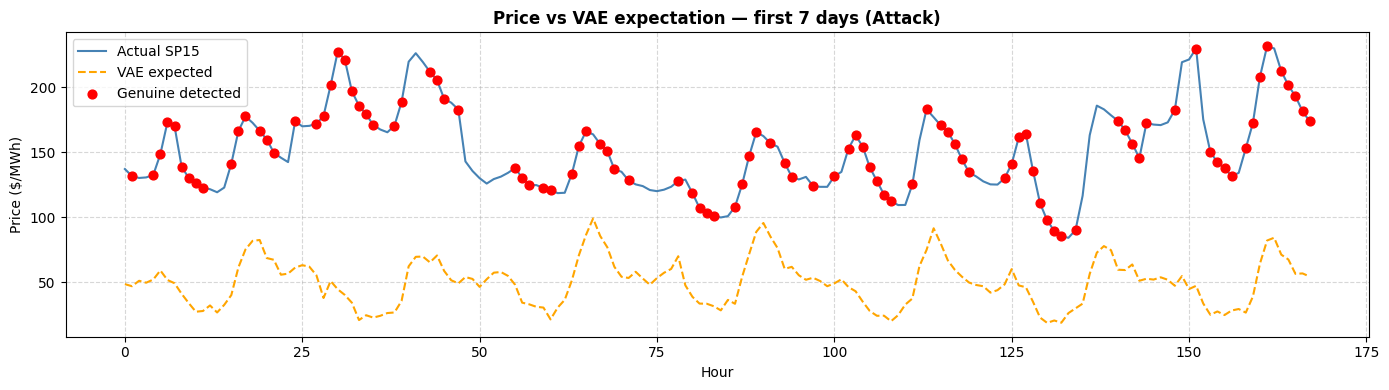
\includegraphics[width=0.475\textwidth]{output.png}
    \caption{SP15 price versus VAE reconstruction for the first 7 days of the attack scenario.}
    \label{fig:output}
\end{figure}

\subsection{Comparison Against State-of-the-Art Methods}
The proposed VAE ensemble was compared against two simpler anomaly detectors within the same opportunistic dispatch pipeline: a rolling z-score threshold and a standalone iForest using continuous outlierness scores. Under attack conditions, the z-score threshold achieves a profit improvement of $-0.98\%$ over baseline, the standalone iForest achieves $+0.27\%$, and the proposed VAE ensemble achieves $+0.53\%$. These results are summarized in Table~\ref{tab:sota}.

The VAE ensemble is the only detector to consistently improve over the baseline in both clean and attack scenarios. The z-score threshold underperforms because it flags legitimate volatility periods as anomalous, causing the optimizer to suppress trades during genuine price events. The iForest alone captures point-level outliers but lacks the temporal coherence of the VAE, leading to noisier anomaly signals. The VAE ensemble's advantage lies in combining temporal structure (VAE), density-level sensitivity (iForest), and local neighborhood context (LOF) into a more reliable $is\_genuine$ score.

\begin{table}[!h]
\centering
\caption{Anomaly Detector Comparison - Opportunistic Dispatch Profit}
\label{tab:sota}
\begin{tabular}{lccc}
\hline
\textbf{Detector} & \textbf{Clean (\$K)} & \textbf{Attack (\$K)} & \textbf{Attack $\Delta$ (\%)} \\
\hline
Threshold (z-score)  & 480.4 & 480.7 & $-0.98$ \\
IsoForest only       & 486.5 & 486.8 & $+0.27$ \\
VAE ensemble (ours)  & 487.7 & 488.0 & $+0.53$ \\
\hline
\end{tabular}
\end{table}
\section{Experimental Setup}

\subsection{Hardware and Software Environment}

The framework was implemented using NumPy and Pandas for data preprocessing, Scikit-Learn for anomaly detection and evaluation, PyTorch for the VAE, and Pyomo with HiGHS for dispatch optimization. Visualization was performed using Matplotlib. Global random seeds (PyTorch, NumPy, Python random, and the Python random module) were set for reproducibility.

The experimental environment is summarized in Table~\ref{tab:hardware}.

\begin{table}[!t]
\centering
\caption{Experimental Computing Environment}
\label{tab:hardware}
\begin{tabular}{ll}
\hline
Component & Specification \\
\hline
Operating System & Windows 11 Home \\
Processor & Intel Core i7-1355U \\
Memory & 16 GB DDR4 \\
Graphics & Intel Iris Xe Graphics \\
Programming Language & Python \\
Development Environment & Visual Studio Code \\
Deep Learning Framework & PyTorch \\
Optimization Framework & Pyomo / HiGHS \\
Machine Learning Library & Scikit-Learn \\
Visualization Library & Matplotlib \\
\hline
\end{tabular}
\end{table}

\subsection{Evaluation Metrics}

The performance of the proposed framework was compared across clean and attack scenarios. VAE reconstruction performance is summarized in Table~\ref{tab:performance_comparison}. Dispatch strategy profits are presented in Table~\ref{tab:strategy_results} and Table~\ref{tab:efc_profit_cycle}.

\begin{table*}[!b]
\centering
\caption{VAE Performance Comparison Between Clean and Attack Scenarios}
\label{tab:performance_comparison}
\begin{tabular}{lccc}
\hline
\textbf{Metric} & \textbf{Clean Scenario} & \textbf{Attack Scenario} & \textbf{Improvement (\%)} \\
\hline
Mean Absolute Error (MAE) [\$/MWh]       & 21.6193 & 20.4828 & $-5.26$ \\
Root Mean Square Error (RMSE) [\$/MWh]   & 32.6332 & 31.5737 & $-3.25$ \\
Coefficient of Determination ($R^2$)     &  0.0625 &  0.1251 & $+100.15$ \\
Final Validation Loss                    &  0.0060 &  0.0038 & $-36.43$ \\
Reconstruction Accuracy [\%]             & 21.5667 & 24.1673 & $+12.06$ \\
\hline
\end{tabular}
\end{table*}

\subsection{Model Configuration}

The VAE model was trained with a 24-hour sequence length and hyperparameter-optimized on a held-out validation split. Twelve candidate configurations were evaluated. The selected parameters are summarized in Table~\ref{tab:vae_config}.

\begin{table}[!t]
\centering
\caption{VAE Training Configuration}
\label{tab:vae_config}
\begin{tabular}{lc}
\hline
\textbf{Parameter} & \textbf{Value} \\
\hline
Epochs                               & 50 \\
Batch Size                           & 16 \\
Learning Rate                        & $1 \times 10^{-3}$ \\
Sequence Length                      & 24 hours \\
Training Fraction                    & 80\% \\
Latent Dimension (Clean)             & 4 \\
Latent Dimension (Attack)            & 4 \\
$\beta$ (Clean)                      & 0.5 \\
$\beta$ (Attack)                     & 0.5 \\
Hyperparameter Configurations Tested & 12 \\
Global Random Seed                   & 42 \\
\hline
\end{tabular}
\end{table}

\section{Limitations}

While the proposed framework demonstrates consistent profit improvement under adversarial conditions, several limitations must be acknowledged. First, the genuine-versus-synthetic classifier currently achieves a synthetic recall of zero within the anomalous-hour evaluation mask, meaning the $is\_genuine$ score does not successfully identify any injected spike as synthetic. Of the 727 anomalous hours evaluated, only 15 correspond to injected spikes; the AUROC of $0.2228$ indicates that the score distribution does not reliably separate the two classes at the current threshold. The practical implication is that the opportunistic regime's profit improvement derives primarily from better exploitation of genuine spikes rather than active avoidance of synthetic ones.

Second, the $\lambda$ sensitivity curve does not exhibit the expected inverted-U behavior in the current evaluation. Opportunistic dispatch profit increases monotonically across the full $\lambda \in [0, 1]$ sweep rather than peaking at an interior optimum. This is a direct consequence of the zero synthetic recall: when no synthetic spikes are penalized, increasing $\lambda$ amplifies the response to genuine spikes only, producing a one-sided effect. A well-calibrated classifier would introduce downward pressure on profit at high $\lambda$ values, recovering the expected peak.

Third, all experiments are conducted exclusively on the SP15 trading hub of the CAISO market. The generalizability of the learned VAE representations and classification thresholds to NP15, ZP26, or markets outside CAISO has not been evaluated.

Fourth, the adversarial injection model is non-adaptive: spikes are injected with fixed statistical properties and do not respond to the detection pipeline. A sophisticated adversary with knowledge of the ensemble's decision boundary could craft injections that evade detection by mimicking genuine market behavior.

\section{Conclusion}

This paper presents an anomaly-aware battery dispatch framework that addresses a practical, underexplored vulnerability in automated energy markets: the exposure of BESS dispatch algorithms to adversarial price-spike injection. The proposed pipeline combines a VAE with iForest and LOF into a three-member ensemble anomaly detector, followed by a behavioral classification stage that assigns each flagged price event a continuous $is\_genuine$ score based on persistence, mean-reversion, and rate-of-change criteria. This score is integrated directly into a linear programming dispatch optimizer operating under three regimes - baseline, penalized, and opportunistic - allowing the system to exploit confirmed genuine spikes while dampening responses to suspected synthetic injections.

Experiments on three years of CAISO SP15 hourly price data spanning January 2023 through December 2025 demonstrate that the opportunistic regime achieves a consistent profit improvement of $0.53\%$ over the anomaly-agnostic baseline under adversarial conditions. The genuine-versus-synthetic classifier achieves an $F_1$ score of $0.5859$ and a precision of $0.9615$ on 727 anomalous hours evaluated against honest spike-mask ground truth. A robustness sweep across 15 spike magnitude and duration configurations with 100 injected spikes each confirms that anomaly detection rate scales from $10.7\%$ at low-severity attacks to $71.0\%$ at high-severity attacks, with profit improvements of $+0.53\%$ to $+1.96\%$ across all configurations. The VAE ensemble outperforms both a z-score threshold baseline ($-0.98\%$) and a standalone iForest ($+0.27\%$) in attack conditions. Explainability is provided through a temporal Grad-CAM adaptation that identifies which hours most influenced the anomaly signal.

Future work will focus on three directions: automated calibration of the $is\_genuine$ threshold using the Youden-J ROC criterion to improve synthetic spike recall; extension to the NP15 and ZP26 trading nodes to evaluate cross-regional generalizability; and evaluation against adaptive adversaries that adjust injection strategies in response to the detection pipeline.

\begin{figure}[!t]
    \centering
    \includegraphics[width=0.475\textwidth]{Sensitivity.png}
    \caption{$\lambda$ sensitivity analysis across both clean and attack scenarios. The opportunistic regime (proposed method) consistently outperforms the baseline across the full range of $\lambda \in [0, 1]$. The penalized regime converges toward a lower bound as $\lambda$ approaches 1.0, reflecting increasing suppression of all anomalous trading.}
    \label{fig:sensitivity}
\end{figure}

\begin{figure}[!t]
    \centering
    \includegraphics[width=0.475\textwidth]{battery.png}
    \caption{Battery SoC over the first 7 days of the attack scenario for the baseline and opportunistic strategies. The opportunistic strategy charges more aggressively during confirmed genuine spike periods, resulting in higher cumulative SOC utilization.}
    \label{fig:battery}
\end{figure}

\begin{figure}[!t]
    \centering
    
\includegraphics[width=0.475\textwidth]{gradcam_week_attack.png}
    \caption{Grad-CAM temporal influence for the most anomalous week in the attack scenario. The shaded area (right axis) shows normalized per-hour VAE influence scores. Hours where the influence score peaks correspond to hours flagged as anomalous, providing a human-readable audit trail for dispatch decisions.}
    \label{fig:gradcam}
\end{figure}

\centering
\caption{Strategy Performance Under Clean and Attack Conditions}
\label{tab:strategy_results}
\begin{tabular}{lcc}
\hline
\textbf{Strategy} & \textbf{Clean (\$K)} & \textbf{Attack (\$K)} \\
\hline
Baseline      & 485.1 & 490.8 \\
Penalized     & 452.4 & 458.6 \\
Opportunistic & 487.7 & 493.4 \\
\hline
\end{tabular}

\vspace{0.5em}

\begin{figure*}[!t]
    \centering
    
\includegraphics[width=0.9\textwidth]{robustness_heatmap.png}
    \caption{Robustness sweep across 15 magnitude - duration configurations, each with 100 injected spikes. Left: anomaly detection rate computed on injected hours only (fraction of spike hours with ensemble score $> 0.15$), showing a clear positive scaling with spike magnitude from $10.7\%$ at $1.5\times$ to $71.0\%$ at $8\times$. Right: opportunistic dispatch profit improvement over baseline (\%), ranging from $+0.53\%$ at low severity to $+1.96\%$ at high severity.}
    \label{fig:robustness}
\end{figure*}

\begin{table*}[!b]
\centering
\caption{Equivalent Full Cycles (EFC) and Profit per Cycle}
\label{tab:efc_profit_cycle}
\begin{tabular}{llccc}
\hline
\textbf{Scenario} & \textbf{Mode} & \textbf{Profit (\$K)} & \textbf{EFC} & \textbf{Profit/Cycle (\$/MWh)} \\
\hline
Clean  & Baseline      & 485.15 & 1229.65 & 394.54 \\
Clean  & Penalized     & 452.44 & 1228.53 & 368.28 \\
Clean  & Opportunistic & 487.74 & 1232.15 & 395.84 \\
Attack & Baseline      & 490.83 & 1235.45 & 397.28 \\
Attack & Penalized     & 458.64 & 1233.52 & 371.82 \\
Attack & Opportunistic & 493.43 & 1237.25 & 398.82 \\
\hline
\end{tabular}
\end{table*}

\bibliographystyle{IEEEtran}
\bibliography{references}
\end{document}